\documentclass[12pt,a4paper]{book}
\usepackage[utf8]{inputenc}
\usepackage[spanish]{babel}
\usepackage{amsmath}
\usepackage{amsfonts}
\usepackage{amssymb}
\usepackage{makeidx}
\usepackage{graphicx}
\usepackage{hyperref}
\usepackage{setspace}
\usepackage{epigraph}
\usepackage{booktabs}
\usepackage[T1]{fontenc}
\usepackage{times}
\usepackage{lipsum}
\renewcommand{\baselinestretch}{2}
\renewcommand{\tablename}{Tabla}
\AtBeginDocument{\renewcommand\tablename{Tabla}}
\usepackage[left=3cm,right=2.5cm,top=3cm,bottom=3cm]{geometry}
\hypersetup{colorlinks,linkcolor={blue},citecolor={blue},urlcolor={red}} 
\title{Calibración de un Prototipo de Detector Cherenkov analizando el Decaimiento del Muón}
\date{Mayo 2021}
\author{Quispe Calloapaza, David Saúl y Quispe Mamani, Sonia Diana}

\begin{document}
	\begin{titlepage}
	\begin{center}
		{\Large \textbf{Universidad Nacional de San Agustín de Arequipa}}\\
		{\Large \textbf{Facultad de Ciencias Naturales y Formales}}\\
		\vspace{1mm}
		{\Large \textbf{Escuela profesional de Física}}\\
		\begin{figure}[h]
			\centering
			
\includegraphics[scale=0.3]{FIGURAS/Logo_unsa.png}
		\end{figure}
		\vspace{1mm}
		\rule{\linewidth}{0.75mm}\\
		\vspace{1mm}
		\begin{spacing}{1.5}
			{\LARGE \textbf{Monitoreo de la estabilidad de respuesta de un prototipo de detector Cherenkov analizando el decaimiento del Muón}}
		\end{spacing}
		\rule{\linewidth}{0.75mm}\\
	\end{center}

    \begin{spacing}{1}
    	\epigraph{Tesis presentada por:\\
    	Quispe Calloapaza, David Saúl\\
    	Quispe Mamani, Sonia Diana\\
    	\vspace{3mm}
    	Para optar el grado de:\\ Bachiller en Física\\
    	\vspace{3mm}
    	Asesores:\\
    	Mg. Rolando Moisés Perca Gonzáles\\
    	Msc. Luis Otiniano Ormachea\\
    	Dr. José Bellido Cáceres}{}
	
	\begin{center}
		Arequipa - Perú\\
		2021
	\end{center}
	\end{spacing}
\end{titlepage}
	
	\tableofcontents
	
	\listoffigures
	
	\chapter{Introducción}
Con la llegada, en 1906, del telescopio óptico de Galileo, se obtuvo el primer avance en las observaciones del universo, que en ese contexto se podían hacer únicamente empleando los ojos de manera directa. Se expandió por primera vez el universo observable para el hombre. Más adelante, nos dimos cuenta que el telescopio era un instrumento limitado para observar el universo, debido a que unicamente podiamos observar la región visible del espectro electromagnético \cite{Vazquez}. Más adelante se emplearían métodos novedosos para observar regiones, del espectro electromagnético, fuera del visible.  

El físico austriaco Víctor Hess entre los años 1911-1912 realizó experimentos cruciales, los cuales ponían en manifiesto la existencia de una radiación cuyo origen era del espacio exterior. Hess publicó los resultados de sus experimentos concluyendo lo siguiente: "Los resultados de estas observaciones parecen poder interpretarse admitiendo sencillamente que una radiación con gran poder de penetración procede de la parte superior de la atmósfera y, aunque progresivamente atenuada por ésta, produce, incluso en las zonas más bajas, una parte de la ionización observada en las cámaras cerradas. La intensidad de está radiación parece estar afectada por pequeñas variaciones aleatorias" \cite{Lugo}.

Hoy en día, se emplean distintos tipos de detectores para poder observar el universo en un rango más amplio de energía, todo esto con el fin de saber lo que hay y como ha ido evolucionando nuestro universo. Los rayos gamma de alta energía, por ejemplo, son producidos en fenómenos llamados GRB (destello de rayos gamma por sus siglas en inglés Gamma Ray Burst) que toman lugar en fenómenos muy violentos en universo como colisión de estrellas masivas, nucleos activos de galaxia, explosiones de estrellas tipo supernova, etc \cite{PEREZY2009}. Por lo que la detección de esta radiación proveniente del espacio exterior nos brinda aún más conocimiento sobre lo sucede en el universo y la evolución de este.
	
	\chapter{Rayos Cósmicos}\label{RAYOS_COSMICOS}
Uno de los rangos de interés para la astrofísica son los rayos cósmicos (CR's por sus siglas en inglés Cosmic Rays) de alta energía. Los CR's consisten en su mayoría de núcleos atómicos ionizados, además de electrones, positrones, antiprotones, rayos gamma y neutrinos que van llegando a la Tierra de algún lugar en el universo, también se les conoce como CRs primarios. Estos CR's se extienden desde poco menos de $1$GeV hasta más allá de los $100$EeV. Con el objetivo de observarlos se han empleado diferentes técnicas de detección dependiendo del rango de energía en estudio.

Por ejemplo, por debajo de pocos cientos de TeV, lo CR's tienen un flujo muy grande de $5\times 10^6$m$^{-2}$sr$^{-1}$yr$^{-1}$, y pueden ser detectado de manera directa por satelites antes de que estos interaccionen con la atmósfera. Pero para CRs con pocos cientos por encima de los TeV el flujo de estos llegan a un valor menor de $50$m$^{-2}$sr$^{-1}$yr$^{-1}$ \cite{MOLLERACH201885}, donde la detección directa ya no es práctica , pues se tendría que tener satélites capaces de abarcar grandes áreas, por lo que se recurren a métodos de detección indirectos que se explicará más adelante. Entonces, la construcción de estaciones de capaces de detectar rayos cósmicos en distintas partes del mundo, brindan información para ampliar el conocimiento del universo observable en astrofísica.

\begin{figure}
	\centering
	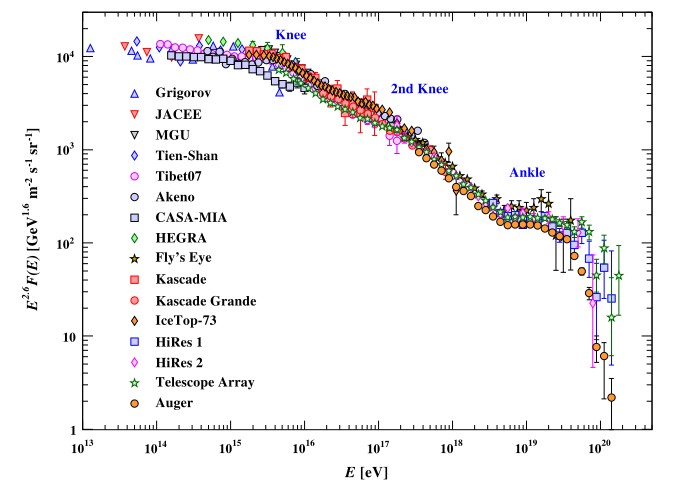
\includegraphics[scale = 0.5]{FIGURAS/ESPECTRO_RC.png}
	\caption{Espectro de flujo de rayos cósmicos a altas energías, multiplicado por $E^{2.6}$ para una mejor observación, en función de la energía \cite{MOLLERACH201885}.}
	\label{Espectro_CR}
\end{figure}

La figura \ref{Espectro_CR}, nos muestra el espectro de flujo de CR's a altas energías, este espectro sigue una ley de potencias de aproximadamente $d\phi /dE \propto E^{-\gamma}$ con un valor de $\gamma \simeq 3$, este espectro muestra algunas interesantes características.
\begin{itemize}
	\item Por encima de pocos cientos de GeV hasta pocos cientos de PeV, el espectro muestra un valor de $\gamma \simeq 2.7$.
	\item En la zona conocida como primera rodilla o ``kne" ($\sim 4 \mbox{PeV}$) el espectro cambia a $\gamma \simeq 3$.
	\item En la zona conocida como segunda rodilla o ``seoncd knee" ($\sim 0.1 \mbox{EeV}$) el espectro cambia a $\gamma \simeq 3.3$.
	\item En la zona concida como tobillo o ``ankle" ($\sim 5 \mbox{EeV}$), el espectro cambia nuevamente con $\gamma \simeq 2.6$.
\end{itemize}

Note que el flujo determinado por varios experimentos varía debido a las técnicas de detección y calibración de energía usado en los distintos experimentos. Además de que, para la detección de CR de altas energías se estudian las cascadas atomosféricas formadas por estos, ver sec. \ref{EAS}.
	
	\chapter{Cascadas atmosféricas y efecto Cherenkov} \label{EAS_Y_CHERENKOV}
\section{Cascadas atmosféricas} \label{EAS}
	Las cascadas atmosféricas (o EAS por sus siglas en inglés Extensive Air Shower) tienen su origen gracias a la interacción de un CR primario, que llega a la Tierra, con la atmósfera terrestre. La mayor parte de estas EAS son iniciadas por CR con energías mayores a $10^{13}$ eV o $10$ TeV. Cuando estos procesos de colisión son dominados por hadrones se forma lo que conoce como cascada hadrónica, que se propaga en la dirección del momento inicial de la partícula primaria. Luego, muones y neutrinos se forman a partir del decaimiento de piones cargados y kaones, formandose también lo que se conoce como cascada muónica.

	\begin{figure}[h]
		\centering
		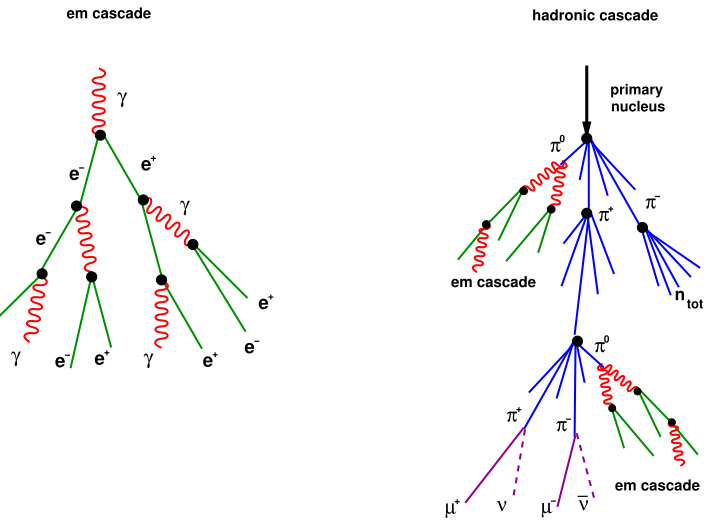
\includegraphics[scale = 0.5]{FIGURAS/CASCADA_LONGITUDINAL.png}
		\caption{Desarrollo longitudinal de una casacada puramente electromagnética y una cascada hadrónica. Los puntos negros representan el lugar de la interacción de la partícula con un núcleo de la atmósfera \cite{MOLLERACH201885}.}
		\label{Cascada_longitudinal}
	\end{figure}

	Los piones neutros y otras partículas decaen en electrones y rayos gamma, formándose así la cascada electromagnética. Aquí se involucran procesos como creación de pares y Bremsstrahlung. De esta manera, una partícula primaria con alta energía puede generar una cascada con gran cantidad de partículas y fotones \cite{GRIEDER2010}.  Dichas cascadas se propagan esencialmente a la velocidad de la luz y pueden alcanzar la superficie terrestre si el CR primario es suficientemenete energético.

	Las cascadas pueden ser iniciadas por hadrones, fotones y electrones, las cascadas iniciadas por fotones o electrones se les conoce como cascadas puramente electromagnéticas. Los fotones de alta energía energía interaccionan con los núcleos de la atmósfera generando la creación de pares $e^+$ y $e^-$, los electrones y positrones interaccionan con los núclos de la atmósfera para porducir fotones mediante Bremsstrahlung \cite{MOLLERACH201885}. A este desarrollo de las cascadas a lo largo de la profundidad atmosférica (medida en gm/cm$^2$) se le conoce como desarrollo longitudinal, la figura \ref{Cascada_longitudinal} nos muestra el desarrollo longitudinal de una cascada puramente electromagnética (inciada por un fotón) y una cascada hadrónica.

\section{Efecto Cherenkov} \label{EFECTO_CHERENKOV}

	
	\bibliographystyle{apalike}
	\bibliography{bibliografia.bib}
\end{document}
